\section*{Recap of Lecture 3}
\phantomsection
\makeatletter
\def\@currentlabel{Recap of Lecture~3}\def\@currentlabelname{Recap of Lecture~3}%
\def\cref@currentlabel{[recap][1][]Recap of Lecture~3}%
\makeatother
\crefformat{recap}{#2#1#3}\Crefformat{recap}{#2#1#3}
\label{sec:recap}
\addcontentsline{toc}{section}{Recap of Lecture 3}

Lecture~3 described how an agent executes. \msa{}, the course's running example, repairs one
reported security weakness at a time: it reads a static-analysis scanner's alert about a file of
OWASP BenchmarkPython, edits the flagged code and submits a patch (Lecture~2). We modeled \msa{}, in its planning version, as an
extended state machine: a machine with finitely many control locations and a set of variables that
its transitions read and write. The planning version, built in Lecture~2, adds a planner and a
validator to the reactive loop, and the Lecture~3 notes call it the planning agent. This recap
restates the terms of that model that recur in this lecture. The Lecture~3 notes, \emph{Execution
machinery and vulnerability triage}, give the full treatment.

\begin{figure*}[t]
  \centering
  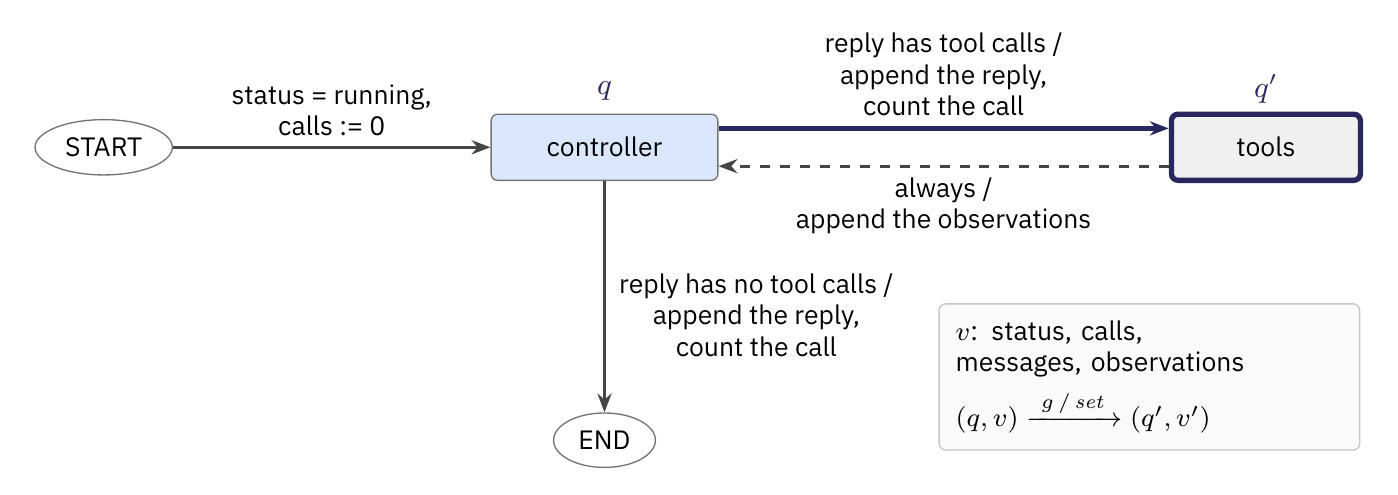
\includegraphics[width=0.8\textwidth]{figures/deck/fc6511c0f9.png}
  \caption{The two-node core of the planning version of \msa{}: the controller, which calls the
  model, and the tools node, which runs the requested tools. Each edge carries its guard and, after
  a slash, its set action, and the highlighted edge is one transition from $(q, v)$ to $(q', v')$.}
  \label{fig:recap-core}
\end{figure*}

A configuration pairs a control location $q$ with the values $v$ of the variables. The control
location is a node of the graph, such as the controller, and it names the computation that runs
next. The variables hold what the run keeps between steps, such as the messages exchanged with the
model and the number of model calls made so far.

Each edge of the graph is a transition. A transition is taken when its guard $g$ holds. The guard of
a transition is a true-or-false test of the variables and of the input that the step received, such
as the model's reply. When the transition is taken, its set action updates $v$. One step therefore
moves the run from a configuration $(q, v)$ to the next configuration $(q', v')$.

The state record stores the values $v$, one named field per variable. A node does not rewrite the
whole record. It returns a partial update, which holds new values only for the fields it changes.
The reducer of each field defines how the returned value is merged with the stored one. For example,
the reducer of \demoref{messages} appends the returned messages to the stored list, and the reducer
of \demoref{model\_calls}, the call count, adds each reported call to the stored total.

An invariant is a property that holds in every reachable configuration, that is, in every
configuration that some run can arrive at from its start. In the planning version, the call budget
gives an invariant: the count of completed model calls never exceeds the budget of 40. The property
holds because each node that calls the model, \demoref{plan}, \demoref{controller} and
\demoref{validate}, checks the count before the call and reports each completed call once.
Lecture~3 called this check the admission check.

Routing functions select the next node. A routing function is code that we write: after a node has
run, it reads the updated record and returns the name of the node that runs next.

A feedback edge sends the run back to a node that it visited earlier. The edge from the tools node
back to the controller, which Lecture~3 called the tool loop, is one example. Each feedback edge has
an explicit bound on how often a run can take it: a limit of its own or the call budget of the whole
run. In the planning version, the plan can be revised at most once per run. The call budget bounds
the other feedback edges, because each of them returns to the controller, which either ends the run
or calls the model.

A trace records one run. Its events show what the machine did, such as the model calls, the tool
requests and their results, and the routing decisions. When the run ends normally, a terminal event
states how it ended. Some moves between nodes have no event of their own and must be inferred.

The trace does not show what those actions did to the files or to anything else outside the
machine. The agent learns about the files only through what its tools report.

\Cref{fig:recap-core} draws the two-node core of the planning version, and the labels on its edges
show when each transition is taken and what it updates. The controller, drawn in blue, calls the
model, and the tools node, drawn in grey, runs the tools that the model requested. The full machine
also has the nodes \demoref{plan}, \demoref{submit} and \demoref{validate}. The figure leaves them
out and draws a reply without tool calls as the end of the run. In the full machine, such a reply
leads to \demoref{submit}, which checks the patch.

Each label gives the guard of the transition, then a slash, then its set action. The figure omits
the output actions, which Lecture~3 defined as the part of a transition that emits an output, such
as a request to run a tool. The arrow from \demoref{START} sets the status to \demoref{running} and
the call count to zero. The box at the bottom right lists the variables in $v$: the status, the call
count (written \emph{calls}), the messages and the observations.

The highlighted edge from the controller to the tools node is one transition from $(q, v)$ to
$(q', v')$. Its guard is that the model's reply has tool calls. Its set action appends the reply to
the messages and counts the call.

The edge from the controller to \demoref{END} has the opposite guard, that the reply has no tool
calls, and the same set action. The two guards exclude each other, because a reply either has tool
calls or has none. Exactly one of the two transitions is therefore taken after each model call.

The dashed edge from the tools node back to the controller is the tool loop. In the figure, its guard
always holds, and its set action appends the observations, the recorded results of the tool calls.

Lecture~3 drew the tools node as one box and treated everything that happens inside it as a single
step. This lecture opens that box, beginning with what a tool call is and which component executes
it (\cref{sec:toolcalls}).
